\documentclass[twoside]{book}

% Packages required by doxygen
\usepackage{fixltx2e}
\usepackage{calc}
\usepackage{doxygen}
\usepackage[export]{adjustbox} % also loads graphicx
\usepackage{graphicx}
\usepackage[utf8]{inputenc}
\usepackage{makeidx}
\usepackage{multicol}
\usepackage{multirow}
\PassOptionsToPackage{warn}{textcomp}
\usepackage{textcomp}
\usepackage[nointegrals]{wasysym}
\usepackage[table]{xcolor}

% Font selection
\usepackage[T1]{fontenc}
\usepackage[scaled=.90]{helvet}
\usepackage{courier}
\usepackage{amssymb}
\usepackage{sectsty}
\renewcommand{\familydefault}{\sfdefault}
\allsectionsfont{%
  \fontseries{bc}\selectfont%
  \color{darkgray}%
}
\renewcommand{\DoxyLabelFont}{%
  \fontseries{bc}\selectfont%
  \color{darkgray}%
}
\newcommand{\+}{\discretionary{\mbox{\scriptsize$\hookleftarrow$}}{}{}}

% Page & text layout
\usepackage{geometry}
\geometry{%
  a4paper,%
  top=2.5cm,%
  bottom=2.5cm,%
  left=2.5cm,%
  right=2.5cm%
}
\tolerance=750
\hfuzz=15pt
\hbadness=750
\setlength{\emergencystretch}{15pt}
\setlength{\parindent}{0cm}
\setlength{\parskip}{3ex plus 2ex minus 2ex}
\makeatletter
\renewcommand{\paragraph}{%
  \@startsection{paragraph}{4}{0ex}{-1.0ex}{1.0ex}{%
    \normalfont\normalsize\bfseries\SS@parafont%
  }%
}
\renewcommand{\subparagraph}{%
  \@startsection{subparagraph}{5}{0ex}{-1.0ex}{1.0ex}{%
    \normalfont\normalsize\bfseries\SS@subparafont%
  }%
}
\makeatother

% Headers & footers
\usepackage{fancyhdr}
\pagestyle{fancyplain}
\fancyhead[LE]{\fancyplain{}{\bfseries\thepage}}
\fancyhead[CE]{\fancyplain{}{}}
\fancyhead[RE]{\fancyplain{}{\bfseries\leftmark}}
\fancyhead[LO]{\fancyplain{}{\bfseries\rightmark}}
\fancyhead[CO]{\fancyplain{}{}}
\fancyhead[RO]{\fancyplain{}{\bfseries\thepage}}
\fancyfoot[LE]{\fancyplain{}{}}
\fancyfoot[CE]{\fancyplain{}{}}
\fancyfoot[RE]{\fancyplain{}{\bfseries\scriptsize Generated by Doxygen }}
\fancyfoot[LO]{\fancyplain{}{\bfseries\scriptsize Generated by Doxygen }}
\fancyfoot[CO]{\fancyplain{}{}}
\fancyfoot[RO]{\fancyplain{}{}}
\renewcommand{\footrulewidth}{0.4pt}
\renewcommand{\chaptermark}[1]{%
  \markboth{#1}{}%
}
\renewcommand{\sectionmark}[1]{%
  \markright{\thesection\ #1}%
}

% Indices & bibliography
\usepackage{natbib}
\usepackage[titles]{tocloft}
\setcounter{tocdepth}{3}
\setcounter{secnumdepth}{5}
\makeindex

% Hyperlinks (required, but should be loaded last)
\usepackage{ifpdf}
\ifpdf
  \usepackage[pdftex,pagebackref=true]{hyperref}
\else
  \usepackage[ps2pdf,pagebackref=true]{hyperref}
\fi
\hypersetup{%
  colorlinks=true,%
  linkcolor=blue,%
  citecolor=blue,%
  unicode%
}

% Custom commands
\newcommand{\clearemptydoublepage}{%
  \newpage{\pagestyle{empty}\cleardoublepage}%
}

\usepackage{caption}
\captionsetup{labelsep=space,justification=centering,font={bf},singlelinecheck=off,skip=4pt,position=top}

%===== C O N T E N T S =====

\begin{document}

% Titlepage & ToC
\hypersetup{pageanchor=false,
             bookmarksnumbered=true,
             pdfencoding=unicode
            }
\pagenumbering{alph}
\begin{titlepage}
\vspace*{7cm}
\begin{center}%
{\Large Biber }\\
\vspace*{1cm}
{\large Generated by Doxygen 1.8.14}\\
\end{center}
\end{titlepage}
\clearemptydoublepage
\pagenumbering{roman}
\tableofcontents
\clearemptydoublepage
\pagenumbering{arabic}
\hypersetup{pageanchor=true}

%--- Begin generated contents ---
\chapter{Hierarchical Index}
\section{Class Hierarchy}
This inheritance list is sorted roughly, but not completely, alphabetically\+:\begin{DoxyCompactList}
\item \contentsline{section}{application.\+Image\+Man}{\pageref{classapplication_1_1_image_man}}{}
\begin{DoxyCompactList}
\item \contentsline{section}{application.\+Blur}{\pageref{classapplication_1_1_blur}}{}
\item \contentsline{section}{application.\+Custom\+Filter}{\pageref{classapplication_1_1_custom_filter}}{}
\item \contentsline{section}{application.\+Edge\+Detection}{\pageref{classapplication_1_1_edge_detection}}{}
\item \contentsline{section}{application.\+Grayscale}{\pageref{classapplication_1_1_grayscale}}{}
\item \contentsline{section}{application.\+Pixel\+Scaling}{\pageref{classapplication_1_1_pixel_scaling}}{}
\item \contentsline{section}{application.\+Threshold}{\pageref{classapplication_1_1_threshold}}{}
\item \contentsline{section}{application.\+Zhang\+Suen}{\pageref{classapplication_1_1_zhang_suen}}{}
\end{DoxyCompactList}
\item \contentsline{section}{application.\+Shared\+Object}{\pageref{classapplication_1_1_shared_object}}{}
\item Application\begin{DoxyCompactList}
\item \contentsline{section}{application.\+Main}{\pageref{classapplication_1_1_main}}{}
\end{DoxyCompactList}
\item Button\begin{DoxyCompactList}
\item \contentsline{section}{application.\+Biber\+Button}{\pageref{classapplication_1_1_biber_button}}{}
\end{DoxyCompactList}
\item Initializable\begin{DoxyCompactList}
\item \contentsline{section}{application.\+F\+X\+Controller}{\pageref{classapplication_1_1_f_x_controller}}{}
\item \contentsline{section}{application.\+F\+X\+Controller2}{\pageref{classapplication_1_1_f_x_controller2}}{}
\end{DoxyCompactList}
\end{DoxyCompactList}

\chapter{Class Index}
\section{Class List}
Here are the classes, structs, unions and interfaces with brief descriptions\+:\begin{DoxyCompactList}
\item\contentsline{section}{\mbox{\hyperlink{classapplication_1_1_blur}{application.\+Blur}} }{\pageref{classapplication_1_1_blur}}{}
\item\contentsline{section}{\mbox{\hyperlink{classapplication_1_1_f_x_controller}{application.\+F\+X\+Controller}} }{\pageref{classapplication_1_1_f_x_controller}}{}
\item\contentsline{section}{\mbox{\hyperlink{classapplication_1_1_f_x_controller2}{application.\+F\+X\+Controller2}} }{\pageref{classapplication_1_1_f_x_controller2}}{}
\item\contentsline{section}{\mbox{\hyperlink{classapplication_1_1_grayscale}{application.\+Grayscale}} }{\pageref{classapplication_1_1_grayscale}}{}
\item\contentsline{section}{\mbox{\hyperlink{classapplication_1_1_image_man}{application.\+Image\+Man}} }{\pageref{classapplication_1_1_image_man}}{}
\item\contentsline{section}{\mbox{\hyperlink{classapplication_1_1_main}{application.\+Main}} }{\pageref{classapplication_1_1_main}}{}
\item\contentsline{section}{\mbox{\hyperlink{classapplication_1_1_shared_object}{application.\+Shared\+Object}} }{\pageref{classapplication_1_1_shared_object}}{}
\item\contentsline{section}{\mbox{\hyperlink{classapplication_1_1_threshold}{application.\+Threshold}} }{\pageref{classapplication_1_1_threshold}}{}
\end{DoxyCompactList}

\chapter{Class Documentation}
\hypertarget{classapplication_1_1_blur}{}\section{application.\+Blur Class Reference}
\label{classapplication_1_1_blur}\index{application.\+Blur@{application.\+Blur}}
Inheritance diagram for application.\+Blur\+:\begin{figure}[H]
\begin{center}
\leavevmode
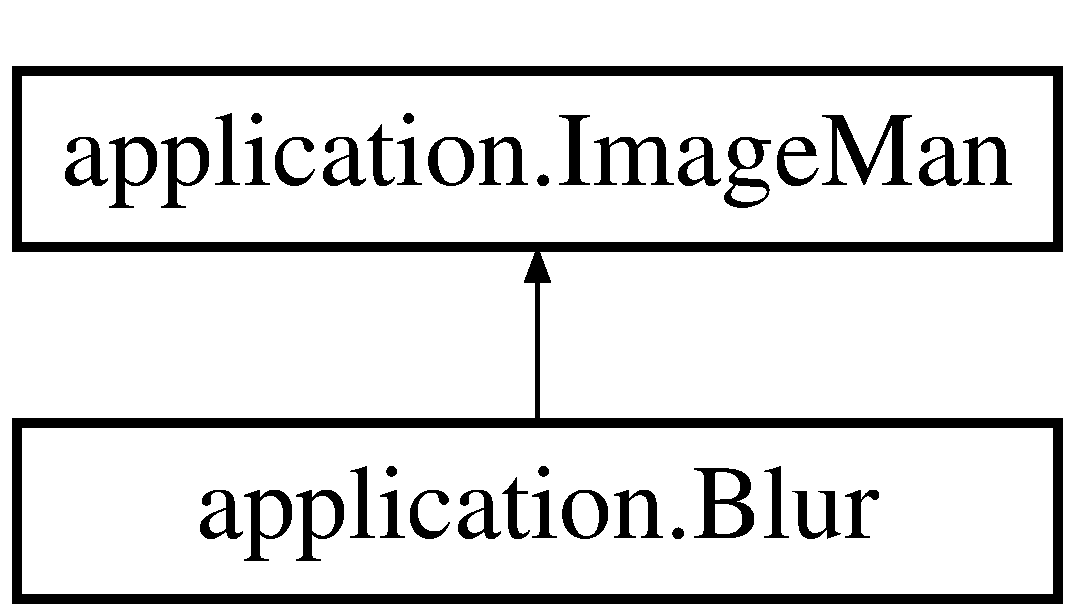
\includegraphics[height=2.000000cm]{classapplication_1_1_blur}
\end{center}
\end{figure}
\subsection*{Public Member Functions}
\begin{DoxyCompactItemize}
\item 
\mbox{\Hypertarget{classapplication_1_1_blur_a11b7920603463fd30f12618d1022caaa}\label{classapplication_1_1_blur_a11b7920603463fd30f12618d1022caaa}} 
{\bfseries Blur} (String ftype, int filterpower)
\item 
\mbox{\Hypertarget{classapplication_1_1_blur_afb919280e2244cf0336ab4a07ee847f6}\label{classapplication_1_1_blur_afb919280e2244cf0336ab4a07ee847f6}} 
{\bfseries Blur} (String ftype, int filterpower, double sigma\+Colour, double sigma\+Space)
\item 
\mbox{\Hypertarget{classapplication_1_1_blur_aaff487804568cdfa1f42b3427ecbec14}\label{classapplication_1_1_blur_aaff487804568cdfa1f42b3427ecbec14}} 
{\bfseries Blur} (Mat src, String ftype, int filterpower, double sigma\+Colour, double sigma\+Space)
\item 
\mbox{\Hypertarget{classapplication_1_1_blur_aae56105de62ef267d249903178237592}\label{classapplication_1_1_blur_aae56105de62ef267d249903178237592}} 
void {\bfseries use\+Filter} ()
\item 
\mbox{\Hypertarget{classapplication_1_1_blur_a73c1dba26db59f9cb006c13b843146c1}\label{classapplication_1_1_blur_a73c1dba26db59f9cb006c13b843146c1}} 
String {\bfseries to\+String} ()
\item 
\mbox{\Hypertarget{classapplication_1_1_blur_ae21240e5551b397eb32ccf136bb851b5}\label{classapplication_1_1_blur_ae21240e5551b397eb32ccf136bb851b5}} 
Buffered\+Image {\bfseries return\+Image} ()
\item 
\mbox{\Hypertarget{classapplication_1_1_blur_a8c8b3cadaf7c42b4fdc15080af7fb4d8}\label{classapplication_1_1_blur_a8c8b3cadaf7c42b4fdc15080af7fb4d8}} 
void {\bfseries set\+Src} (Mat src)
\item 
\mbox{\Hypertarget{classapplication_1_1_blur_ab1533310fb2826fb7ca663e10937101f}\label{classapplication_1_1_blur_ab1533310fb2826fb7ca663e10937101f}} 
Mat {\bfseries get\+Dst} ()
\item 
\mbox{\Hypertarget{classapplication_1_1_blur_ae17dd6e4aea39a1d7b7b027f597a7f2b}\label{classapplication_1_1_blur_ae17dd6e4aea39a1d7b7b027f597a7f2b}} 
String {\bfseries get\+Ftype} ()
\item 
\mbox{\Hypertarget{classapplication_1_1_blur_ac1eb14c472923aa1e228f9b7da5e0723}\label{classapplication_1_1_blur_ac1eb14c472923aa1e228f9b7da5e0723}} 
Mat {\bfseries get\+Src} ()
\item 
\mbox{\Hypertarget{classapplication_1_1_blur_a0bab9619fb6330aa2026f006de3f2257}\label{classapplication_1_1_blur_a0bab9619fb6330aa2026f006de3f2257}} 
void {\bfseries set\+Dst} (Mat dst)
\item 
\mbox{\Hypertarget{classapplication_1_1_blur_a5c8e0528528b0b0dda9aaf9b0980e848}\label{classapplication_1_1_blur_a5c8e0528528b0b0dda9aaf9b0980e848}} 
void {\bfseries set\+Ftype} (String ftype)
\item 
Mat \mbox{\hyperlink{classapplication_1_1_blur_a445cba49c071e6a84b9ae6d56f208f60}{gaussian\+Blur}} (Mat src, int filter\+Power)
\item 
Mat \mbox{\hyperlink{classapplication_1_1_blur_a070e2c5803f62149b71ae9bc867a44da}{median\+Blur}} (Mat src, int filter\+Power)
\item 
Mat \mbox{\hyperlink{classapplication_1_1_blur_aa26cb7151a1acda73884d3fb9479e971}{homogen\+Blur}} (Mat src, int filter\+Power)
\item 
Mat \mbox{\hyperlink{classapplication_1_1_blur_af85191ef064d33c47886bc17d6af9ebe}{bilateral\+Blur}} (Mat src, int filter\+Power, double sigma\+Colour, double sigma\+Space)
\end{DoxyCompactItemize}


\subsection{Detailed Description}
Blurring (smoothing) is the commonly used image processing operation for reducing the image noise. The process removes high-\/frequency content, like edges, from the image and makes it smooth. In general blurring is achieved by convolving (each element of the image is added to its local neighbors, weighted by the kernel) the image through a low pass filter kernel.

src\+: The source (input image) for this operation. dst\+: The destination (output image) for this operation. sigma\+Color\+: Filter sigma in the color space. sigma\+Space\+: Filter sigma in the coordinate space. Size( w, h )\+: Defines the size of the kernel to be used ( of width w pixels and height h pixels). Point(-\/1, -\/1)\+: Indicates where the anchor point (the pixel evaluated) is located with respect to the neighborhood. If there is a negative value, then the center of the kernel is considered the anchor point. 

\subsection{Member Function Documentation}
\mbox{\Hypertarget{classapplication_1_1_blur_af85191ef064d33c47886bc17d6af9ebe}\label{classapplication_1_1_blur_af85191ef064d33c47886bc17d6af9ebe}} 
\index{application\+::\+Blur@{application\+::\+Blur}!bilateral\+Blur@{bilateral\+Blur}}
\index{bilateral\+Blur@{bilateral\+Blur}!application\+::\+Blur@{application\+::\+Blur}}
\subsubsection{\texorpdfstring{bilateral\+Blur()}{bilateralBlur()}}
{\footnotesize\ttfamily Mat application.\+Blur.\+bilateral\+Blur (\begin{DoxyParamCaption}\item[{Mat}]{src,  }\item[{int}]{filter\+Power,  }\item[{double}]{sigma\+Colour,  }\item[{double}]{sigma\+Space }\end{DoxyParamCaption})}

The Bilateral Filter operation applies a bilateral image to a filter. \mbox{\Hypertarget{classapplication_1_1_blur_a445cba49c071e6a84b9ae6d56f208f60}\label{classapplication_1_1_blur_a445cba49c071e6a84b9ae6d56f208f60}} 
\index{application\+::\+Blur@{application\+::\+Blur}!gaussian\+Blur@{gaussian\+Blur}}
\index{gaussian\+Blur@{gaussian\+Blur}!application\+::\+Blur@{application\+::\+Blur}}
\subsubsection{\texorpdfstring{gaussian\+Blur()}{gaussianBlur()}}
{\footnotesize\ttfamily Mat application.\+Blur.\+gaussian\+Blur (\begin{DoxyParamCaption}\item[{Mat}]{src,  }\item[{int}]{filter\+Power }\end{DoxyParamCaption})}

Gaussian filtering is done by convolving each point in the input array with a Gaussian kernel and then summing them all to produce the output array. The Gaussian filter is a low-\/pass filter that removes the high-\/frequency components are reduced. \mbox{\Hypertarget{classapplication_1_1_blur_aa26cb7151a1acda73884d3fb9479e971}\label{classapplication_1_1_blur_aa26cb7151a1acda73884d3fb9479e971}} 
\index{application\+::\+Blur@{application\+::\+Blur}!homogen\+Blur@{homogen\+Blur}}
\index{homogen\+Blur@{homogen\+Blur}!application\+::\+Blur@{application\+::\+Blur}}
\subsubsection{\texorpdfstring{homogen\+Blur()}{homogenBlur()}}
{\footnotesize\ttfamily Mat application.\+Blur.\+homogen\+Blur (\begin{DoxyParamCaption}\item[{Mat}]{src,  }\item[{int}]{filter\+Power }\end{DoxyParamCaption})}

Open\+CV offers the function blur to perform smoothing with this filter. \mbox{\Hypertarget{classapplication_1_1_blur_a070e2c5803f62149b71ae9bc867a44da}\label{classapplication_1_1_blur_a070e2c5803f62149b71ae9bc867a44da}} 
\index{application\+::\+Blur@{application\+::\+Blur}!median\+Blur@{median\+Blur}}
\index{median\+Blur@{median\+Blur}!application\+::\+Blur@{application\+::\+Blur}}
\subsubsection{\texorpdfstring{median\+Blur()}{medianBlur()}}
{\footnotesize\ttfamily Mat application.\+Blur.\+median\+Blur (\begin{DoxyParamCaption}\item[{Mat}]{src,  }\item[{int}]{filter\+Power }\end{DoxyParamCaption})}

The median filter run through each element of the signal (in this case the image) and replace each pixel with the median of its neighboring pixels (located in a square neighborhood around the evaluated pixel). 

The documentation for this class was generated from the following file\+:\begin{DoxyCompactItemize}
\item 
D\+:/\+Git/\+S\+W\+Prakt\+S\+S18/\+G\+U\+I/src/application/Blur.\+java\end{DoxyCompactItemize}

\hypertarget{classapplication_1_1_f_x_controller}{}\section{application.\+F\+X\+Controller Class Reference}
\label{classapplication_1_1_f_x_controller}\index{application.\+F\+X\+Controller@{application.\+F\+X\+Controller}}
Inheritance diagram for application.\+F\+X\+Controller\+:\begin{figure}[H]
\begin{center}
\leavevmode
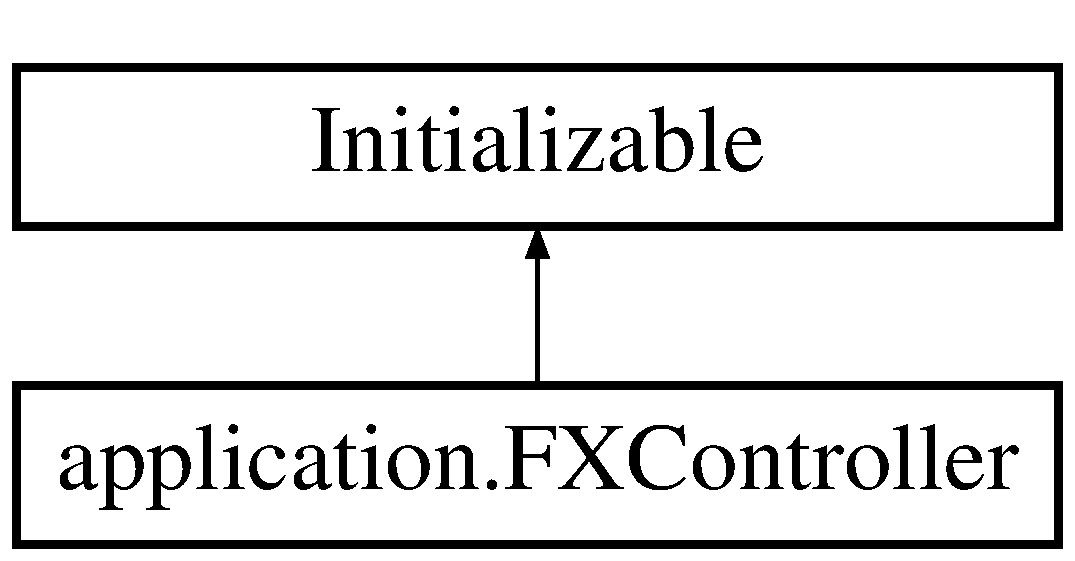
\includegraphics[height=2.000000cm]{classapplication_1_1_f_x_controller}
\end{center}
\end{figure}
\subsection*{Public Member Functions}
\begin{DoxyCompactItemize}
\item 
void \mbox{\hyperlink{classapplication_1_1_f_x_controller_ac94b73f4dcdad256b2e4d5314dc42d2b}{handle\+About}} (Action\+Event event)
\item 
\mbox{\Hypertarget{classapplication_1_1_f_x_controller_a1aa99fad0d86d829a852e17712a5029a}\label{classapplication_1_1_f_x_controller_a1aa99fad0d86d829a852e17712a5029a}} 
void {\bfseries initialize} (U\+RL arg0, Resource\+Bundle arg1)
\item 
\mbox{\Hypertarget{classapplication_1_1_f_x_controller_a4d01b51192bec48b553421fac2adce0e}\label{classapplication_1_1_f_x_controller_a4d01b51192bec48b553421fac2adce0e}} 
void {\bfseries init} (Stage stage)
\item 
void \mbox{\hyperlink{classapplication_1_1_f_x_controller_a46a8c8b397699390607ad6bff526d386}{open\+File}} ()
\item 
void \mbox{\hyperlink{classapplication_1_1_f_x_controller_ae830da008c5d032e83dd11b075f4e9bf}{do\+Exit}} ()
\item 
void \mbox{\hyperlink{classapplication_1_1_f_x_controller_a723312c2219263bdfadd98d86186a365}{choose\+Image}} (Action\+Event event)
\item 
void \mbox{\hyperlink{classapplication_1_1_f_x_controller_af9d560a93b56e46e95d267e0e4b205a2}{save\+File}} ()
\item 
\mbox{\Hypertarget{classapplication_1_1_f_x_controller_aa7ab2bfcf354e8919ea10ff7c4477e1b}\label{classapplication_1_1_f_x_controller_aa7ab2bfcf354e8919ea10ff7c4477e1b}} 
void {\bfseries handle\+Anwenden} (Action\+Event event)
\item 
void \mbox{\hyperlink{classapplication_1_1_f_x_controller_a4ba7818448465dabfafce77571565fb7}{handle\+Window}} (Action\+Event event2)
\end{DoxyCompactItemize}


\subsection{Member Function Documentation}
\mbox{\Hypertarget{classapplication_1_1_f_x_controller_a723312c2219263bdfadd98d86186a365}\label{classapplication_1_1_f_x_controller_a723312c2219263bdfadd98d86186a365}} 
\index{application\+::\+F\+X\+Controller@{application\+::\+F\+X\+Controller}!choose\+Image@{choose\+Image}}
\index{choose\+Image@{choose\+Image}!application\+::\+F\+X\+Controller@{application\+::\+F\+X\+Controller}}
\subsubsection{\texorpdfstring{choose\+Image()}{chooseImage()}}
{\footnotesize\ttfamily void application.\+F\+X\+Controller.\+choose\+Image (\begin{DoxyParamCaption}\item[{Action\+Event}]{event }\end{DoxyParamCaption})}

This method will allow the user to import an image. \mbox{\Hypertarget{classapplication_1_1_f_x_controller_ae830da008c5d032e83dd11b075f4e9bf}\label{classapplication_1_1_f_x_controller_ae830da008c5d032e83dd11b075f4e9bf}} 
\index{application\+::\+F\+X\+Controller@{application\+::\+F\+X\+Controller}!do\+Exit@{do\+Exit}}
\index{do\+Exit@{do\+Exit}!application\+::\+F\+X\+Controller@{application\+::\+F\+X\+Controller}}
\subsubsection{\texorpdfstring{do\+Exit()}{doExit()}}
{\footnotesize\ttfamily void application.\+F\+X\+Controller.\+do\+Exit (\begin{DoxyParamCaption}{ }\end{DoxyParamCaption})}

This method will close the window. \mbox{\Hypertarget{classapplication_1_1_f_x_controller_ac94b73f4dcdad256b2e4d5314dc42d2b}\label{classapplication_1_1_f_x_controller_ac94b73f4dcdad256b2e4d5314dc42d2b}} 
\index{application\+::\+F\+X\+Controller@{application\+::\+F\+X\+Controller}!handle\+About@{handle\+About}}
\index{handle\+About@{handle\+About}!application\+::\+F\+X\+Controller@{application\+::\+F\+X\+Controller}}
\subsubsection{\texorpdfstring{handle\+About()}{handleAbout()}}
{\footnotesize\ttfamily void application.\+F\+X\+Controller.\+handle\+About (\begin{DoxyParamCaption}\item[{Action\+Event}]{event }\end{DoxyParamCaption})}

About Biber. This method opens a new window, which provides brief information about the program. \mbox{\Hypertarget{classapplication_1_1_f_x_controller_a4ba7818448465dabfafce77571565fb7}\label{classapplication_1_1_f_x_controller_a4ba7818448465dabfafce77571565fb7}} 
\index{application\+::\+F\+X\+Controller@{application\+::\+F\+X\+Controller}!handle\+Window@{handle\+Window}}
\index{handle\+Window@{handle\+Window}!application\+::\+F\+X\+Controller@{application\+::\+F\+X\+Controller}}
\subsubsection{\texorpdfstring{handle\+Window()}{handleWindow()}}
{\footnotesize\ttfamily void application.\+F\+X\+Controller.\+handle\+Window (\begin{DoxyParamCaption}\item[{Action\+Event}]{event2 }\end{DoxyParamCaption})}

This method contains the second window to see the changes in the image. \mbox{\Hypertarget{classapplication_1_1_f_x_controller_a46a8c8b397699390607ad6bff526d386}\label{classapplication_1_1_f_x_controller_a46a8c8b397699390607ad6bff526d386}} 
\index{application\+::\+F\+X\+Controller@{application\+::\+F\+X\+Controller}!open\+File@{open\+File}}
\index{open\+File@{open\+File}!application\+::\+F\+X\+Controller@{application\+::\+F\+X\+Controller}}
\subsubsection{\texorpdfstring{open\+File()}{openFile()}}
{\footnotesize\ttfamily void application.\+F\+X\+Controller.\+open\+File (\begin{DoxyParamCaption}{ }\end{DoxyParamCaption})}

This method will open an file. The file formats available to the user are P\+NG and J\+P\+G2000. Loading the image\mbox{\Hypertarget{classapplication_1_1_f_x_controller_af9d560a93b56e46e95d267e0e4b205a2}\label{classapplication_1_1_f_x_controller_af9d560a93b56e46e95d267e0e4b205a2}} 
\index{application\+::\+F\+X\+Controller@{application\+::\+F\+X\+Controller}!save\+File@{save\+File}}
\index{save\+File@{save\+File}!application\+::\+F\+X\+Controller@{application\+::\+F\+X\+Controller}}
\subsubsection{\texorpdfstring{save\+File()}{saveFile()}}
{\footnotesize\ttfamily void application.\+F\+X\+Controller.\+save\+File (\begin{DoxyParamCaption}{ }\end{DoxyParamCaption})}

This method will save an file. The file formats available to the user are P\+NG and J\+P\+G2000. 

The documentation for this class was generated from the following file\+:\begin{DoxyCompactItemize}
\item 
D\+:/\+Git/\+S\+W\+Prakt\+S\+S18/\+G\+U\+I/src/application/F\+X\+Controller.\+java\end{DoxyCompactItemize}

\hypertarget{classapplication_1_1_f_x_controller2}{}\section{application.\+F\+X\+Controller2 Class Reference}
\label{classapplication_1_1_f_x_controller2}\index{application.\+F\+X\+Controller2@{application.\+F\+X\+Controller2}}
Inheritance diagram for application.\+F\+X\+Controller2\+:\begin{figure}[H]
\begin{center}
\leavevmode
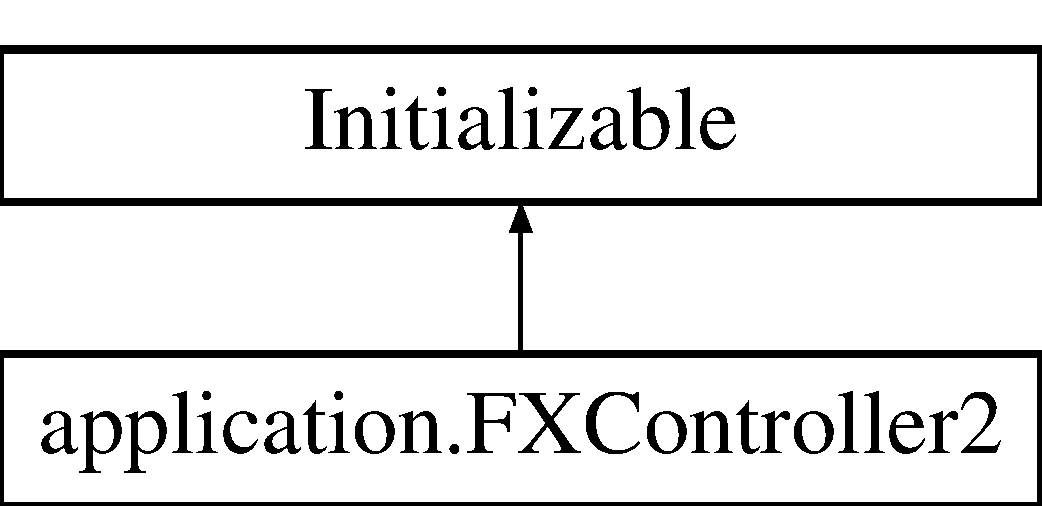
\includegraphics[height=2.000000cm]{classapplication_1_1_f_x_controller2}
\end{center}
\end{figure}
\subsection*{Public Member Functions}
\begin{DoxyCompactItemize}
\item 
\mbox{\Hypertarget{classapplication_1_1_f_x_controller2_aabd0ecbee219d6d3a79147a5d1b3fd06}\label{classapplication_1_1_f_x_controller2_aabd0ecbee219d6d3a79147a5d1b3fd06}} 
void {\bfseries set\+Image} (Image img)
\item 
\mbox{\Hypertarget{classapplication_1_1_f_x_controller2_a889afcc4017257a1e172adb2ce87350a}\label{classapplication_1_1_f_x_controller2_a889afcc4017257a1e172adb2ce87350a}} 
void {\bfseries set\+Image\+In\+Image\+View} ()
\item 
\mbox{\Hypertarget{classapplication_1_1_f_x_controller2_aa4a46ed76cd926e4d37fdd3e4fe8092e}\label{classapplication_1_1_f_x_controller2_aa4a46ed76cd926e4d37fdd3e4fe8092e}} 
void {\bfseries initialize} (U\+RL location, Resource\+Bundle resources)
\end{DoxyCompactItemize}


\subsection{Detailed Description}
Passes the original image and the current image.

The \mbox{\hyperlink{classapplication_1_1_f_x_controller2}{F\+X\+Controller2}} provides the original image and the currently edited image to be able to compare them in a separate window. The original image is obtained via the class \mbox{\hyperlink{classapplication_1_1_shared_object}{Shared\+Object}} in which a singleton pattern was realized and the currently edited image from the \mbox{\hyperlink{classapplication_1_1_f_x_controller}{F\+X\+Controller}}. 

The documentation for this class was generated from the following file\+:\begin{DoxyCompactItemize}
\item 
D\+:/\+Git/\+S\+W\+Prakt\+S\+S18/\+G\+U\+I/src/application/F\+X\+Controller2.\+java\end{DoxyCompactItemize}

\hypertarget{classapplication_1_1_grayscale}{}\section{application.\+Grayscale Class Reference}
\label{classapplication_1_1_grayscale}\index{application.\+Grayscale@{application.\+Grayscale}}
Inheritance diagram for application.\+Grayscale\+:\begin{figure}[H]
\begin{center}
\leavevmode
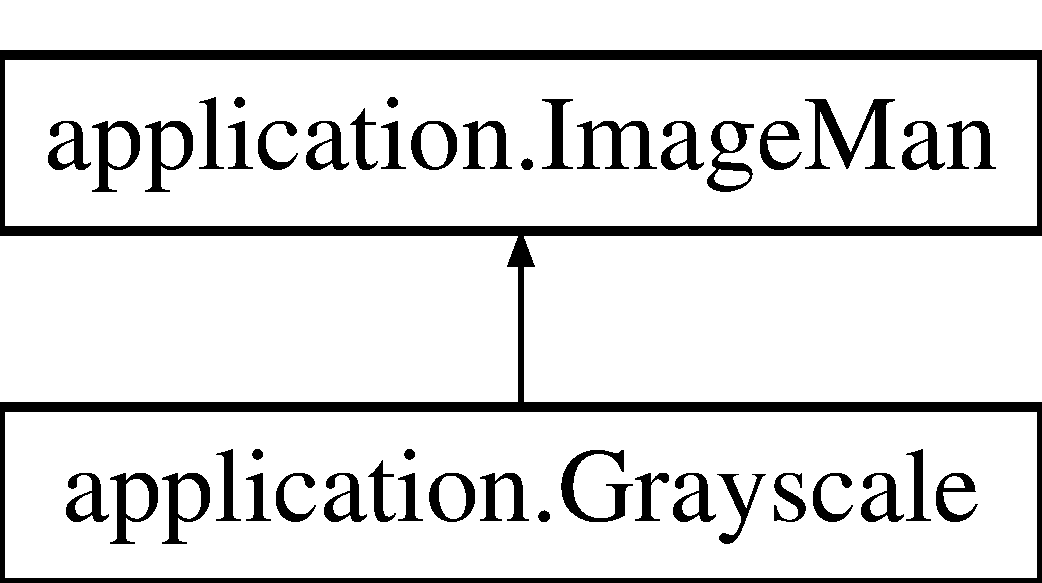
\includegraphics[height=2.000000cm]{classapplication_1_1_grayscale}
\end{center}
\end{figure}
\subsection*{Public Member Functions}
\begin{DoxyCompactItemize}
\item 
\mbox{\Hypertarget{classapplication_1_1_grayscale_a6bf7ea7c89bcc25fa1f2ef43583a3bdb}\label{classapplication_1_1_grayscale_a6bf7ea7c89bcc25fa1f2ef43583a3bdb}} 
Mat {\bfseries luminosity} (Mat src)
\item 
\mbox{\Hypertarget{classapplication_1_1_grayscale_a4fecb13f22f5d72062ce164cf0a491ed}\label{classapplication_1_1_grayscale_a4fecb13f22f5d72062ce164cf0a491ed}} 
Mat {\bfseries gray\+Pixel} (int row, int col, Mat mat)
\item 
\mbox{\Hypertarget{classapplication_1_1_grayscale_a3ef991beb69461c85a1c6bbf706e0605}\label{classapplication_1_1_grayscale_a3ef991beb69461c85a1c6bbf706e0605}} 
Mat {\bfseries average} (Mat src)
\item 
\mbox{\Hypertarget{classapplication_1_1_grayscale_a7b371c1462bfa33b5cf1b491cead7ba4}\label{classapplication_1_1_grayscale_a7b371c1462bfa33b5cf1b491cead7ba4}} 
Mat {\bfseries lightness} (Mat src)
\end{DoxyCompactItemize}


The documentation for this class was generated from the following file\+:\begin{DoxyCompactItemize}
\item 
D\+:/\+Git/\+S\+W\+Prakt\+S\+S18/\+G\+U\+I/src/application/Grayscale.\+java\end{DoxyCompactItemize}

\hypertarget{classapplication_1_1_image_man}{}\section{application.\+Image\+Man Class Reference}
\label{classapplication_1_1_image_man}\index{application.\+Image\+Man@{application.\+Image\+Man}}
Inheritance diagram for application.\+Image\+Man\+:\begin{figure}[H]
\begin{center}
\leavevmode
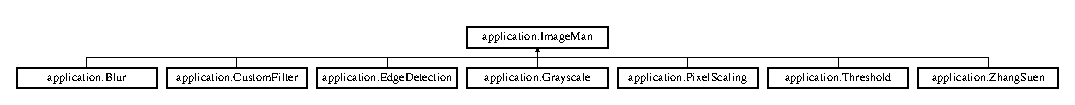
\includegraphics[height=2.000000cm]{classapplication_1_1_image_man}
\end{center}
\end{figure}
\subsection*{Public Member Functions}
\begin{DoxyCompactItemize}
\item 
\mbox{\Hypertarget{classapplication_1_1_image_man_aae0baacc6ca5c01021d2045a6cd3b2c7}\label{classapplication_1_1_image_man_aae0baacc6ca5c01021d2045a6cd3b2c7}} 
Buffered\+Image {\bfseries mat\+To\+Buff\+Image} (Mat m)
\item 
\mbox{\Hypertarget{classapplication_1_1_image_man_aaa60d625c007f0cd250b92359c396287}\label{classapplication_1_1_image_man_aaa60d625c007f0cd250b92359c396287}} 
Mat {\bfseries buff\+Image\+To\+Mat} (Buffered\+Image img)
\end{DoxyCompactItemize}


The documentation for this class was generated from the following file\+:\begin{DoxyCompactItemize}
\item 
D\+:/\+Git/\+S\+W\+Prakt\+S\+S18/\+G\+U\+I/src/application/Image\+Man.\+java\end{DoxyCompactItemize}

\hypertarget{classapplication_1_1_main}{}\section{application.\+Main Class Reference}
\label{classapplication_1_1_main}\index{application.\+Main@{application.\+Main}}
Inheritance diagram for application.\+Main\+:\begin{figure}[H]
\begin{center}
\leavevmode
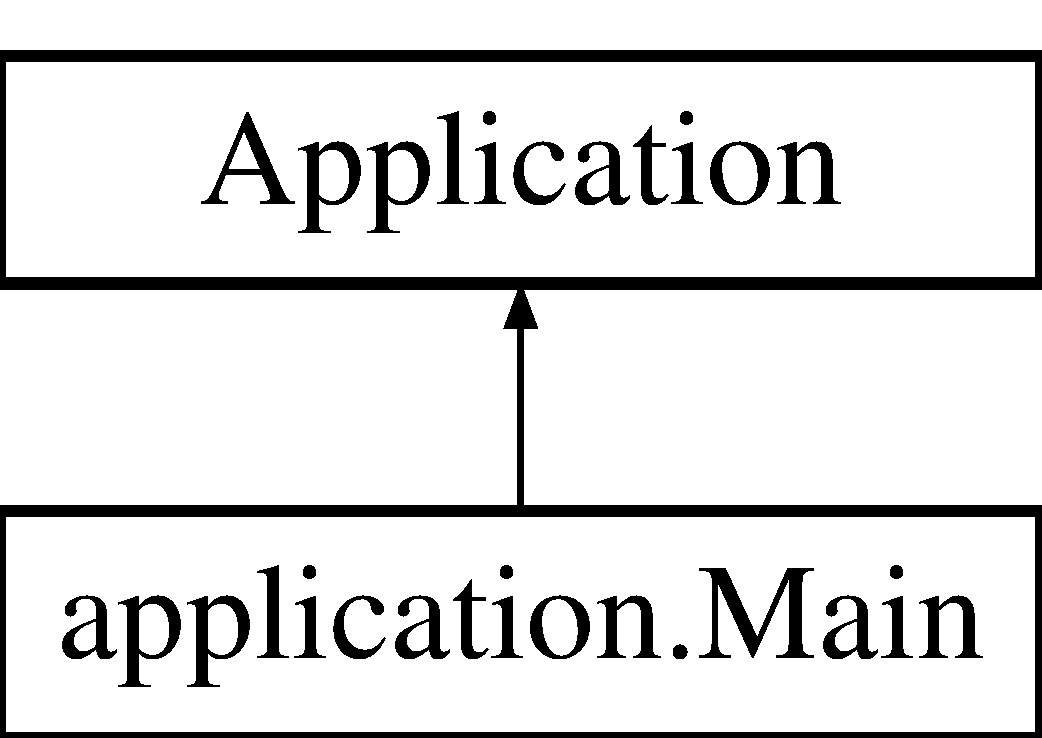
\includegraphics[height=2.000000cm]{classapplication_1_1_main}
\end{center}
\end{figure}
\subsection*{Public Member Functions}
\begin{DoxyCompactItemize}
\item 
\mbox{\Hypertarget{classapplication_1_1_main_a4e5ad4e3de8bbd8654120180a94e870d}\label{classapplication_1_1_main_a4e5ad4e3de8bbd8654120180a94e870d}} 
void {\bfseries start} (Stage primary\+Stage)  throws Exception
\end{DoxyCompactItemize}
\subsection*{Static Public Member Functions}
\begin{DoxyCompactItemize}
\item 
\mbox{\Hypertarget{classapplication_1_1_main_a0de7d10858e36e34a0836c2c6c02c4fc}\label{classapplication_1_1_main_a0de7d10858e36e34a0836c2c6c02c4fc}} 
static void {\bfseries main} (String\mbox{[}$\,$\mbox{]} args)
\end{DoxyCompactItemize}


The documentation for this class was generated from the following file\+:\begin{DoxyCompactItemize}
\item 
D\+:/\+Git/\+S\+W\+Prakt\+S\+S18/\+G\+U\+I/src/application/Main.\+java\end{DoxyCompactItemize}

\hypertarget{classapplication_1_1_shared_object}{}\section{application.\+Shared\+Object Class Reference}
\label{classapplication_1_1_shared_object}\index{application.\+Shared\+Object@{application.\+Shared\+Object}}
\subsection*{Public Member Functions}
\begin{DoxyCompactItemize}
\item 
\mbox{\Hypertarget{classapplication_1_1_shared_object_a089d7d6170ca682281e9b1da46144f12}\label{classapplication_1_1_shared_object_a089d7d6170ca682281e9b1da46144f12}} 
Image {\bfseries get\+Original\+Image} ()
\item 
\mbox{\Hypertarget{classapplication_1_1_shared_object_a9fb756f502b97ba6a9743717866b1927}\label{classapplication_1_1_shared_object_a9fb756f502b97ba6a9743717866b1927}} 
void {\bfseries set\+Original\+Image} (Image original\+Image)
\end{DoxyCompactItemize}
\subsection*{Static Public Member Functions}
\begin{DoxyCompactItemize}
\item 
\mbox{\Hypertarget{classapplication_1_1_shared_object_a35417b0510f7b9ebf85ac1656ed005ff}\label{classapplication_1_1_shared_object_a35417b0510f7b9ebf85ac1656ed005ff}} 
static \mbox{\hyperlink{classapplication_1_1_shared_object}{Shared\+Object}} {\bfseries get\+Instance} ()
\end{DoxyCompactItemize}


\subsection{Detailed Description}
The \mbox{\hyperlink{classapplication_1_1_shared_object}{Shared\+Object}} contains all Elements that should be accessable within different classes. To reduce the memory overhead this class is implemented as a singelton. 

The documentation for this class was generated from the following file\+:\begin{DoxyCompactItemize}
\item 
D\+:/\+Git/\+S\+W\+Prakt\+S\+S18/\+G\+U\+I/src/application/Shared\+Object.\+java\end{DoxyCompactItemize}

\hypertarget{classapplication_1_1_threshold}{}\section{application.\+Threshold Class Reference}
\label{classapplication_1_1_threshold}\index{application.\+Threshold@{application.\+Threshold}}
Inheritance diagram for application.\+Threshold\+:\begin{figure}[H]
\begin{center}
\leavevmode
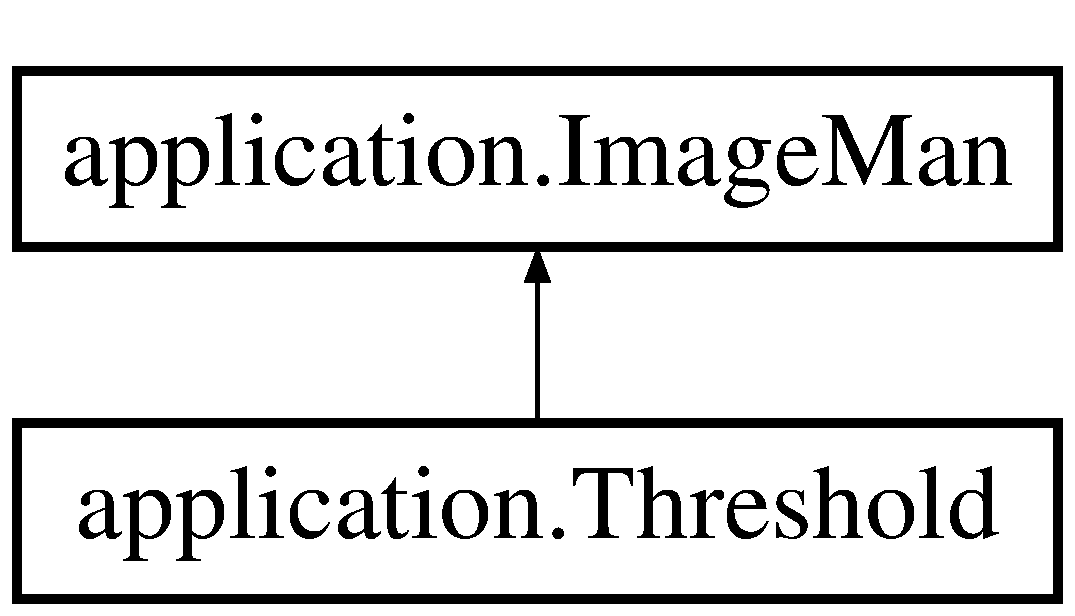
\includegraphics[height=2.000000cm]{classapplication_1_1_threshold}
\end{center}
\end{figure}
\subsection*{Public Member Functions}
\begin{DoxyCompactItemize}
\item 
\mbox{\Hypertarget{classapplication_1_1_threshold_a3711413d5eb746e666aef1ea102b111b}\label{classapplication_1_1_threshold_a3711413d5eb746e666aef1ea102b111b}} 
Mat {\bfseries binarisieren} (int t, Mat src)
\end{DoxyCompactItemize}


The documentation for this class was generated from the following file\+:\begin{DoxyCompactItemize}
\item 
D\+:/\+Git/\+S\+W\+Prakt\+S\+S18/\+G\+U\+I/src/application/Threshold.\+java\end{DoxyCompactItemize}

%--- End generated contents ---

% Index
\backmatter
\newpage
\phantomsection
\clearemptydoublepage
\addcontentsline{toc}{chapter}{Index}
\printindex

\end{document}
